
\section{Prefect}

Een eerste tool waarvan een Proof of Concept gemaakt wordt is Prefect. Dit zal, in combinatie met MLFlow, gebruikt worden voor het lokaal uitvoeren van Machine Learning pipelines. Hierbij worden alle aanpassingen in de code van het framework vergeleken met de originele code van opdracht 3 van opleidingsonderdeel Machine Learning Operations.

\subsection{Installatie}

De installatie van Prefect gebeurt met de package manager \texttt{pip}. Via de terminal kan Prefect met het volgende commando geïnstalleerd worden, dit zal ook alle benodigde packages installeren:


\begin{minted}{bash}
    pip install -r "requirements_Prefect.txt"
\end{minted}

Om alleen Prefect te installeren kan dit met het volgende \texttt{pip} commando:

\begin{minted}{bash}
    pip install prefect
\end{minted}

\subsection{Lokale Server}

Prefect heeft de mogelijkheid om Machine Learning pipelines lokaal uit te voeren, dit gebeurt met behulp van een lokale server. Deze server kan worden opgestart met het commando:

\begin{minted}{bash}
    prefect server start
\end{minted}

Na het uitvoeren van het startcommando zou het resultaat van Figuur~\ref{fig:Prefect_server} te zien moeten zijn.
\begin{figure}
    \centering
    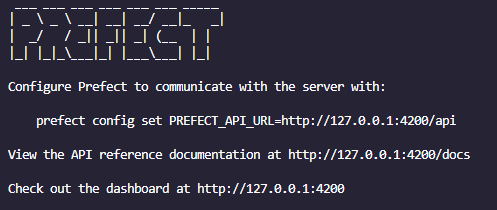
\includegraphics[width=0.9\linewidth]{graphics/Prefect_server.PNG}
    \caption{Uitvoer van de Prefect Server}
    \label{fig:Prefect_server}
\end{figure}

Nu de server is opgestart, moet de code nog communiceren met de Prefect webinterface. Zoals Figuur~\ref{fig:Prefect_server} aantoont, wordt dit gedaan aan de hand van een commando dat gebruikmaakt van een lokale API:

\begin{minted}{bash}
    prefect config set PREFECT_API_URL=http://127.0.0.1:4200/api
\end{minted}

Nu de server opgestart en verbonden is met de lokale omgeving, kan via de ingestelde link het Prefect dashboard worden bezocht.

\subsection{Dashboard}

Het dashboard van Prefect is een omgeving waarin alle pipeline flows worden beheerd. Figuur~\ref{fig:Prefect_Dashboard} geeft een voorbeeld van het Prefect dashboard.

\begin{figure}
    \centering
    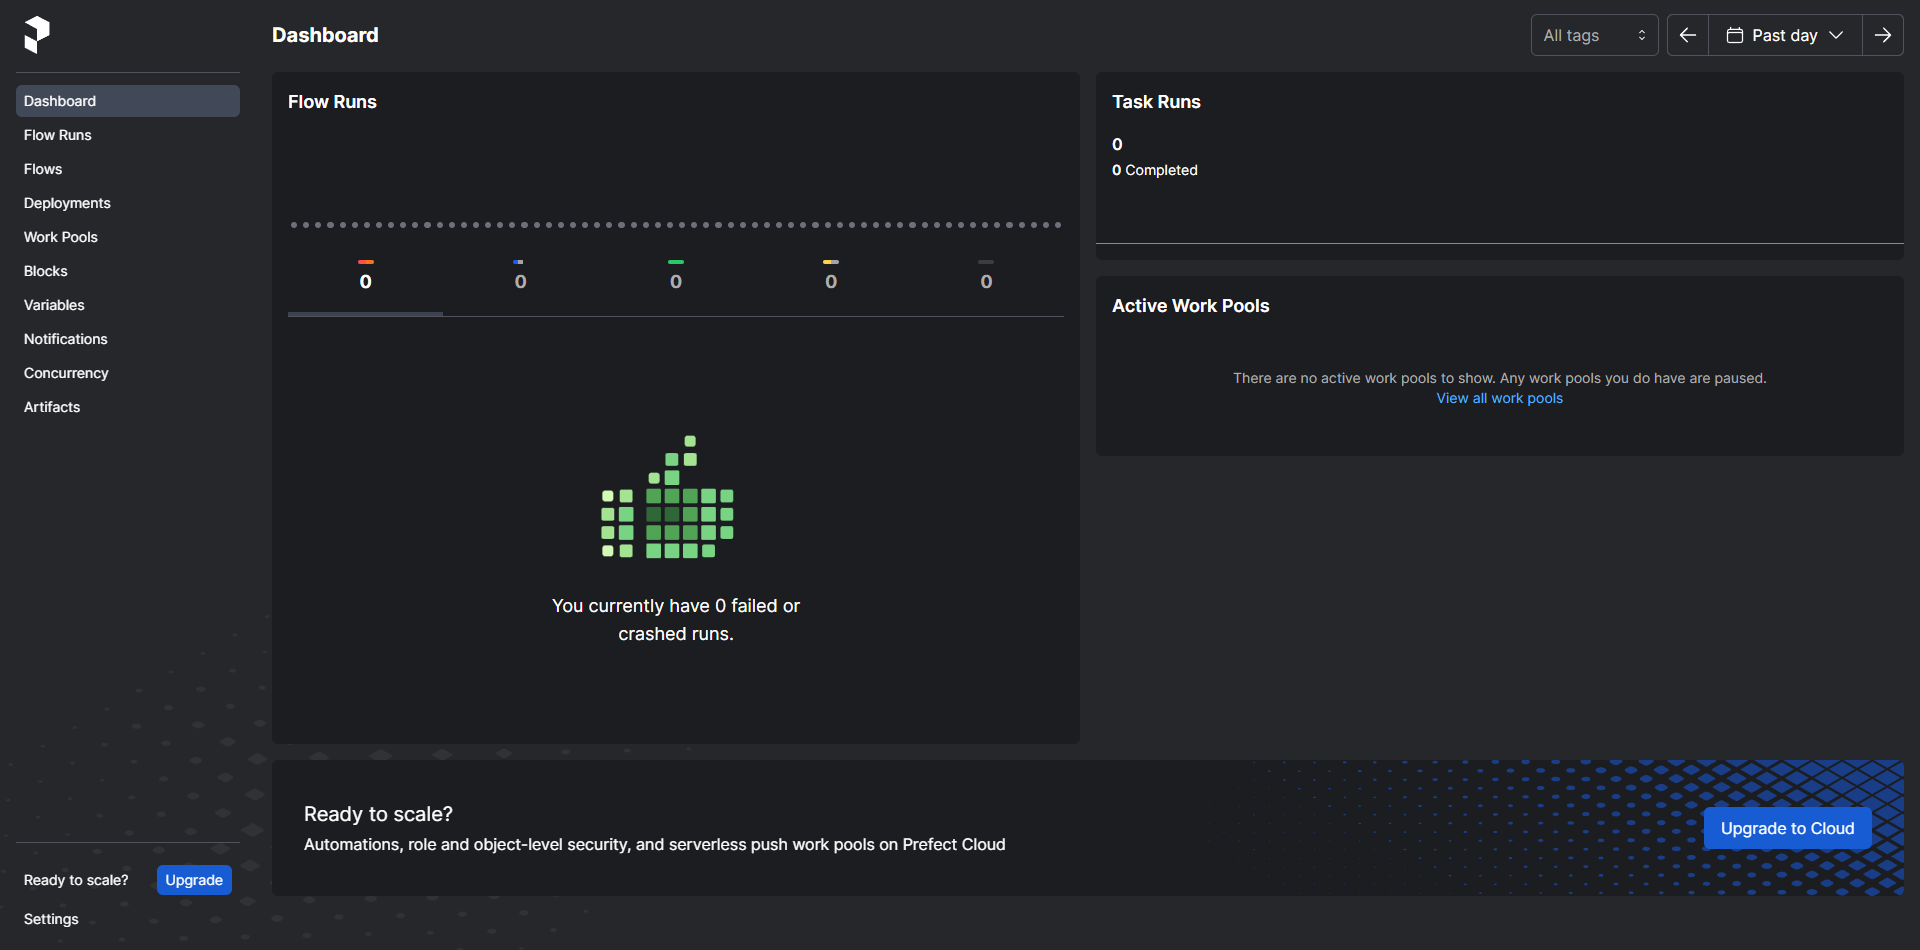
\includegraphics[width=0.9\linewidth]{graphics/Prefect_dashboard.PNG}
    \caption{Voorbeeld van het Prefect Dashboard}
    \label{fig:Prefect_Dashboard}
\end{figure}

De functies die kunnen worden gezien op Figuur~\ref{fig:Prefect_Dashboard} zijn:

\begin{itemize}
    \item \textbf{Dashboard:} Geeft een overzicht van alle flow runs. Hier kan worden bekeken wanneer een flow succesvol of onsuccesvol is uitgevoerd.
    \item \textbf{Flow Runs:} Geeft een tijdlijn weer met alle flows die uitgevoerd zijn over een bepaalde tijd.
    \item \textbf{Flows:} Toont elke flow aan die in de code is geschreven. Hierbij kan ook in de flow gekeken worden om te zien welke taken het bevat.
    \item \textbf{Deployments:} Geeft alle deployments weer. Dit zijn flows die rechtstreeks met het dashboard kunnen worden uitgevoerd.
    \item \textbf{Blocks:} Hier wordt alle gevoelige informatie bijgehouden, zoals wachtwoorden en API keys.
    \item \textbf{Work Pools:} Hier kan verbinding gemaakt worden met een cloud omgeving om de pipeline daar te laten uitvoeren.
\end{itemize}

Deze Proof of Concept zal gebruik maken van de \textit{Flow runs} en \textit{Flows} pagina's op het dashboard.

\subsection{Uitvoering}

Prefect werkt met decorators. Dit zorgt ervoor dat bestaande Python-functies eenvoudig kunnen worden omgezet naar het Prefect framework. De twee decorators \texttt{@task} en \texttt{@flow} werden eerder in de Sectie~\ref{subsec:prefect} besproken. Deze maken het mogelijk om bestaande Python functies om te zetten naar het Prefect framework.

Origineel bevatte het preprocessinggedeelte het downloaden en het verwerken van de afbeeldingen. Echter, voor het uitvoeren in Prefect werd dit nog eens onderverdeeld in twee aparte delen. Het downloaden en het verwerken van de afbeeldingen gebeurt dus apart. De volledige code van de pipeline is te vinden in de GitHub-repository van deze Proof of Concept. % TODO: refereer naar dezelfde voetnoot hier

De download functie werd een \texttt{Task} de andere functies werden een \texttt{Flow}. Dit werd gedaan door de decorators voor de functie te plaatsen. Uiteindelijk worden dan alle \texttt{Tasks} en \texttt{Flows} samengevoegd in één pipeline.

\subsubsection{Pipeline}

De pipeline in Prefect is een flow waarin alle taken en flows achter elkaar worden uitgevoerd. De flow of pipeline ziet er als volgt uit:

\begin{minted}[frame=lines,breaklines,linenos]{python}
@flow(task_runner=SequentialTaskRunner(), log_prints=True)
def main():
    tracking_uri = "http://127.0.0.1:8080"
    model_name = "PoC"
    mlflow.set_tracking_uri(tracking_uri)
    mlflow.set_experiment(model_name)
    download()
    preprocess()
    model = train()
    eval(model)
\end{minted}

Deze code stelt eerst het juiste tracking adres in voor MLflow, alsook de modelnaam. Hierna worden alle functies achter elkaar uitgevoerd en kunnen deze dan ook in de dashboard gezien worden.

In dit geval heeft de \texttt{@flow} nog extra parameters, deze betekenen:

\begin{itemize}
    \item \texttt{task\_runner}: Geeft aan hoe de taken en flows moeten uitgevoerd worden. In dit geval is dat een \texttt{SequentialTaskRunner} wat betekent dat alle tasks en flows achter elkaar worden uitgevoerd.
    \item \texttt{log\_prints}: Geeft alle prints weer die in de Python code werden gebruikt. In dit geval is de waarde \texttt{True}. Dit maakt het debuggen eenvoudig tijden het ontwikkelen van de pipeline.
\end{itemize}

Na het uitvoeren van de flow word deze flow gevisualiseerd in de web interface van Prefect. Figuur~\ref{fig:Prefect_Flow} toont hoe deze pagina in Prefect eruit ziet.
\begin{figure}
    \centering
    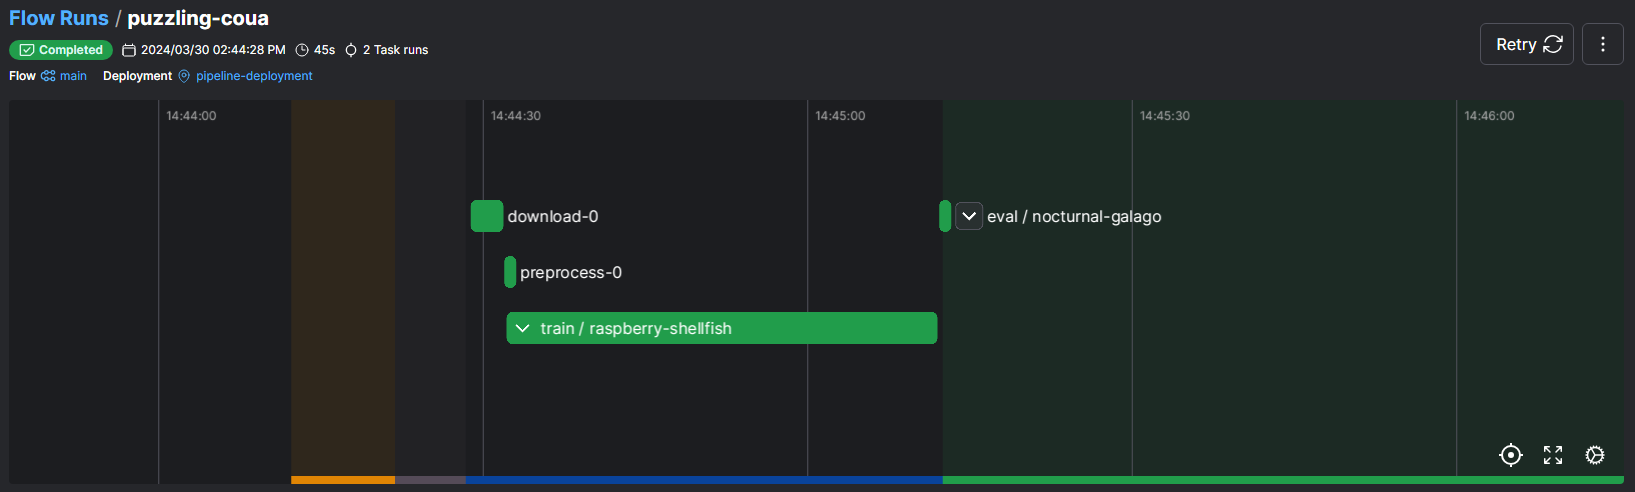
\includegraphics[width=0.9\linewidth]{graphics/Prefect_Flow.PNG}
    \caption{Flow gevisualiseerd in Prefect}
    \label{fig:Prefect_Flow}
\end{figure}

\subsection{Problemen}

Prefect had moeite met het doorgeven van parameters naar de volgende task, waardoor de flow niet meer kon werken. Om dit op te lossen werd er gebruik gemaakt van een subflow. Subflows zijn flows die worden uitgevoerd in een bestaande flow. Deze ontvangen wel goed de parameters en kunnen alles goed uitvoeren.

\subsection{Cloud}

Prefect heeft een concept genaamd \textit{Work Pools}. Figuur~\ref{fig:Prefect_Work_Pools} toont hoe deze pagina in Prefect eruit ziet.

\begin{figure}
    \centering
    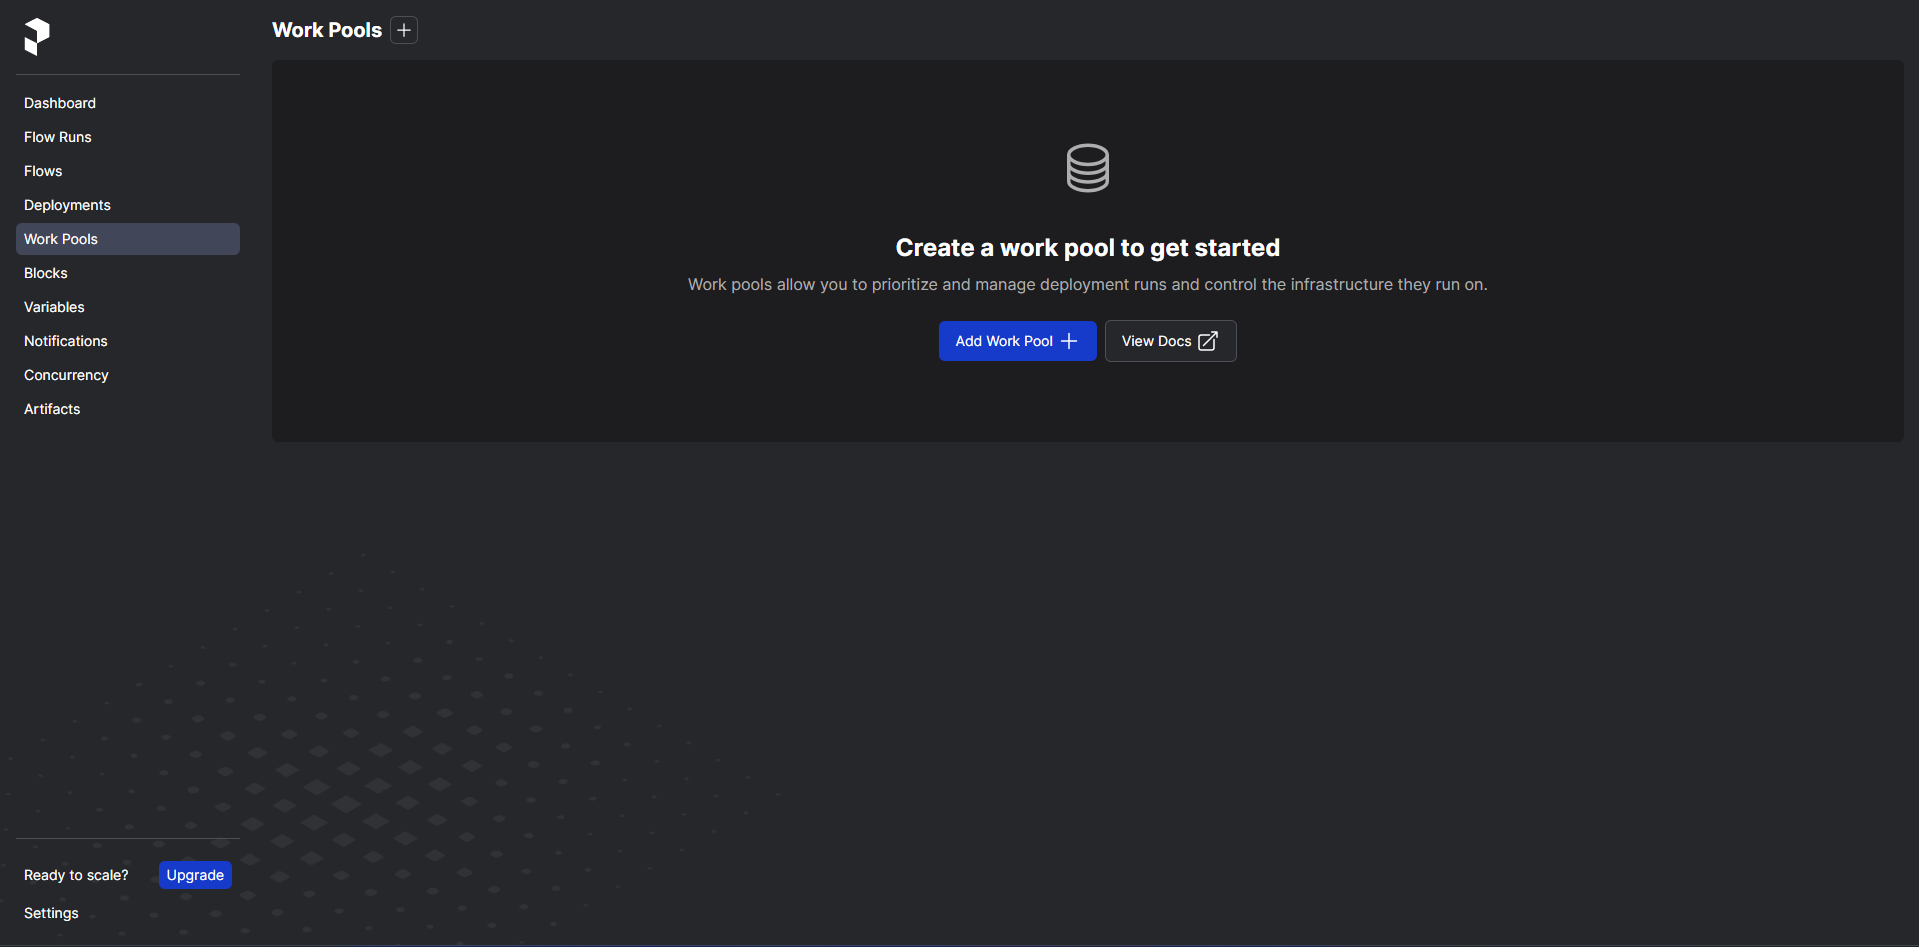
\includegraphics[width=0.9\linewidth]{graphics/Prefect_Work_Pools.PNG}
    \caption{Voorbeeld van de Prefect Work Pool pagina}
    \label{fig:Prefect_Work_Pools}
\end{figure}

Op deze pagina kan er een work pool worden toegevoegd. Dit zorgt voor een verbinding met een cloud omgeving, zodat de Prefect flow in de cloud kan worden uitgevoerd. Het aanmaken van een verbinding kan via de knop \texttt{Add Work Pool}, zoals te zien is op Figuur~\ref{fig:Prefect_Work_Pools}.

Na het klikken op deze knop kan de gewenste cloudomgeving gekozen worden (zie Figuur~\ref{fig:Prefect_Work_Pools_Create}).

\begin{figure}
    \centering
    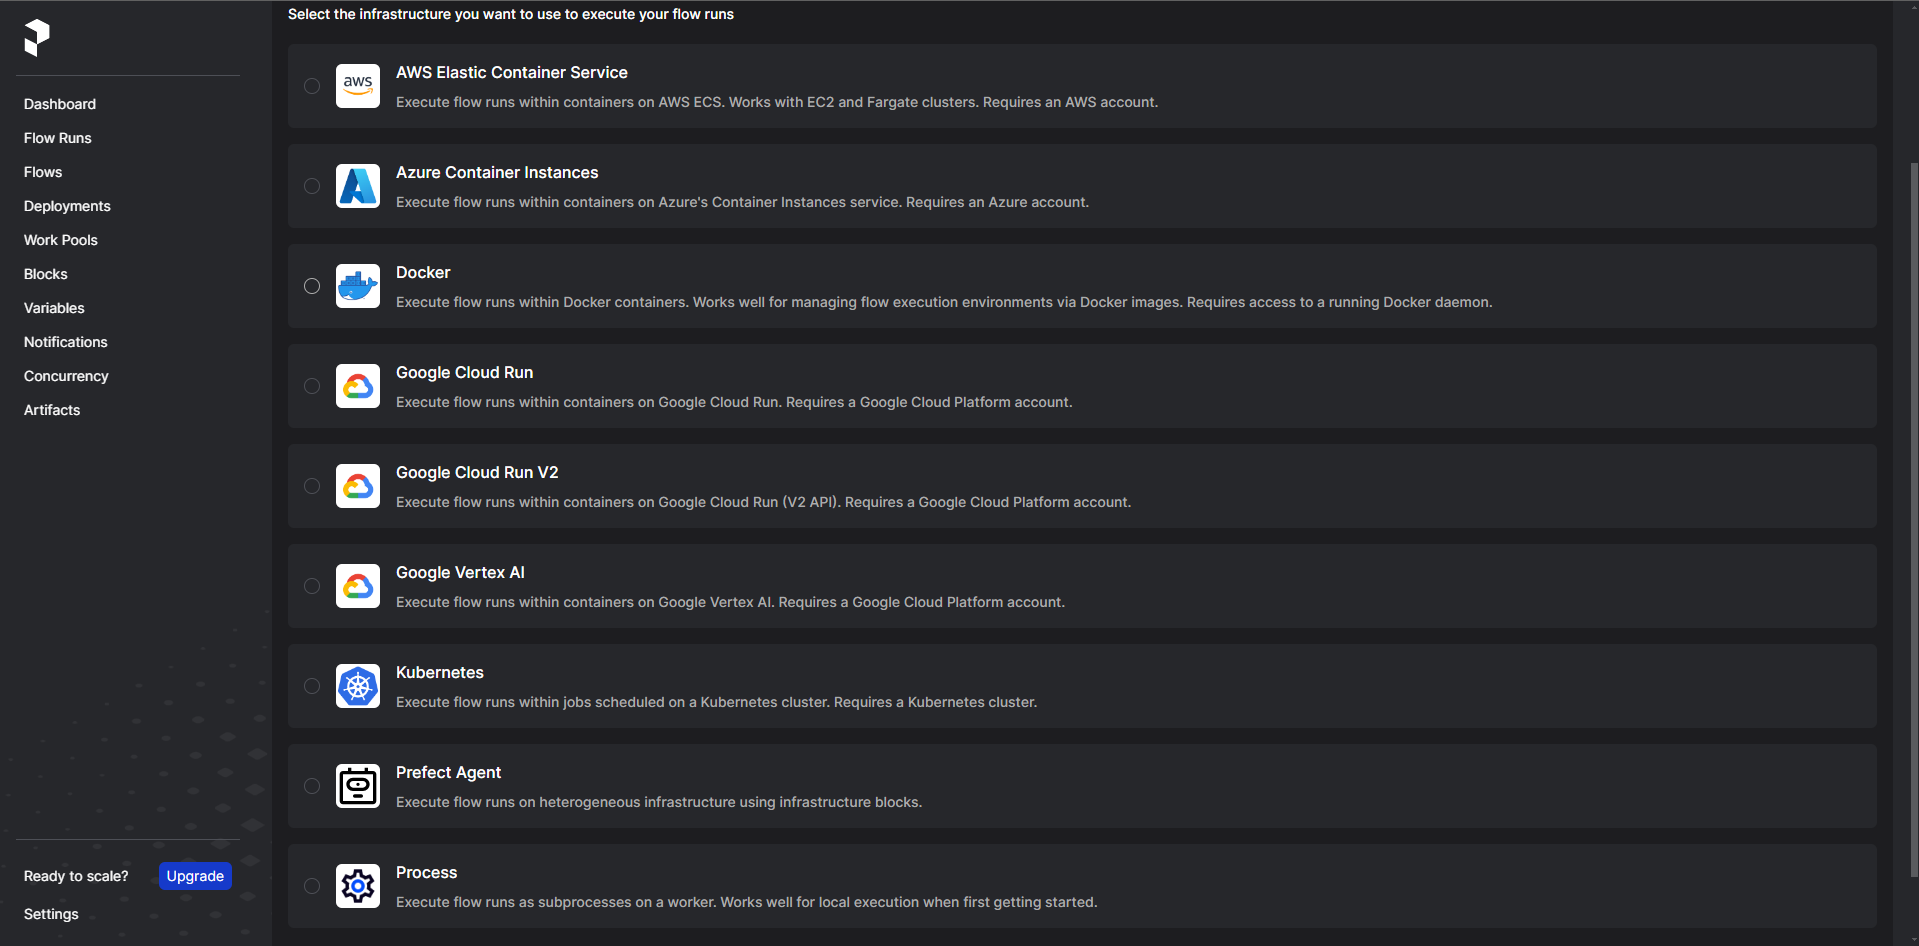
\includegraphics[width=0.9\linewidth]{graphics/Prefect_Work_Pools_Create.PNG}
    \caption{Mogelijke cloud omgevingen voor Prefect Work Pools}
    \label{fig:Prefect_Work_Pools_Create}
\end{figure}

Figuur~\ref{fig:Prefect_Work_Pools_Create} toont de verschillende cloud omgevingen waarmee Prefect kan werken. Deze omvatten onder andere AWS Elastic Container Service, Azure Container Instances, Docker, Google Cloud Run (v2), Google Vertex AI, Kubernetes, Prefect Agent en Process.

In dit voorbeeld wordt \texttt{Process} geselecteerd omdat er momenteel geen toegang is tot een cloudomgeving. De volgende stap is het invullen van details. Deze details zijn de naam en de beschrijving van de work pool en eventuele concurrency. Alleen de naam is verplicht in te vullen, zoals te zien is op Figuur~\ref{fig:Prefect_Work_Pools_Create_Details}.

\begin{figure}
    \centering
    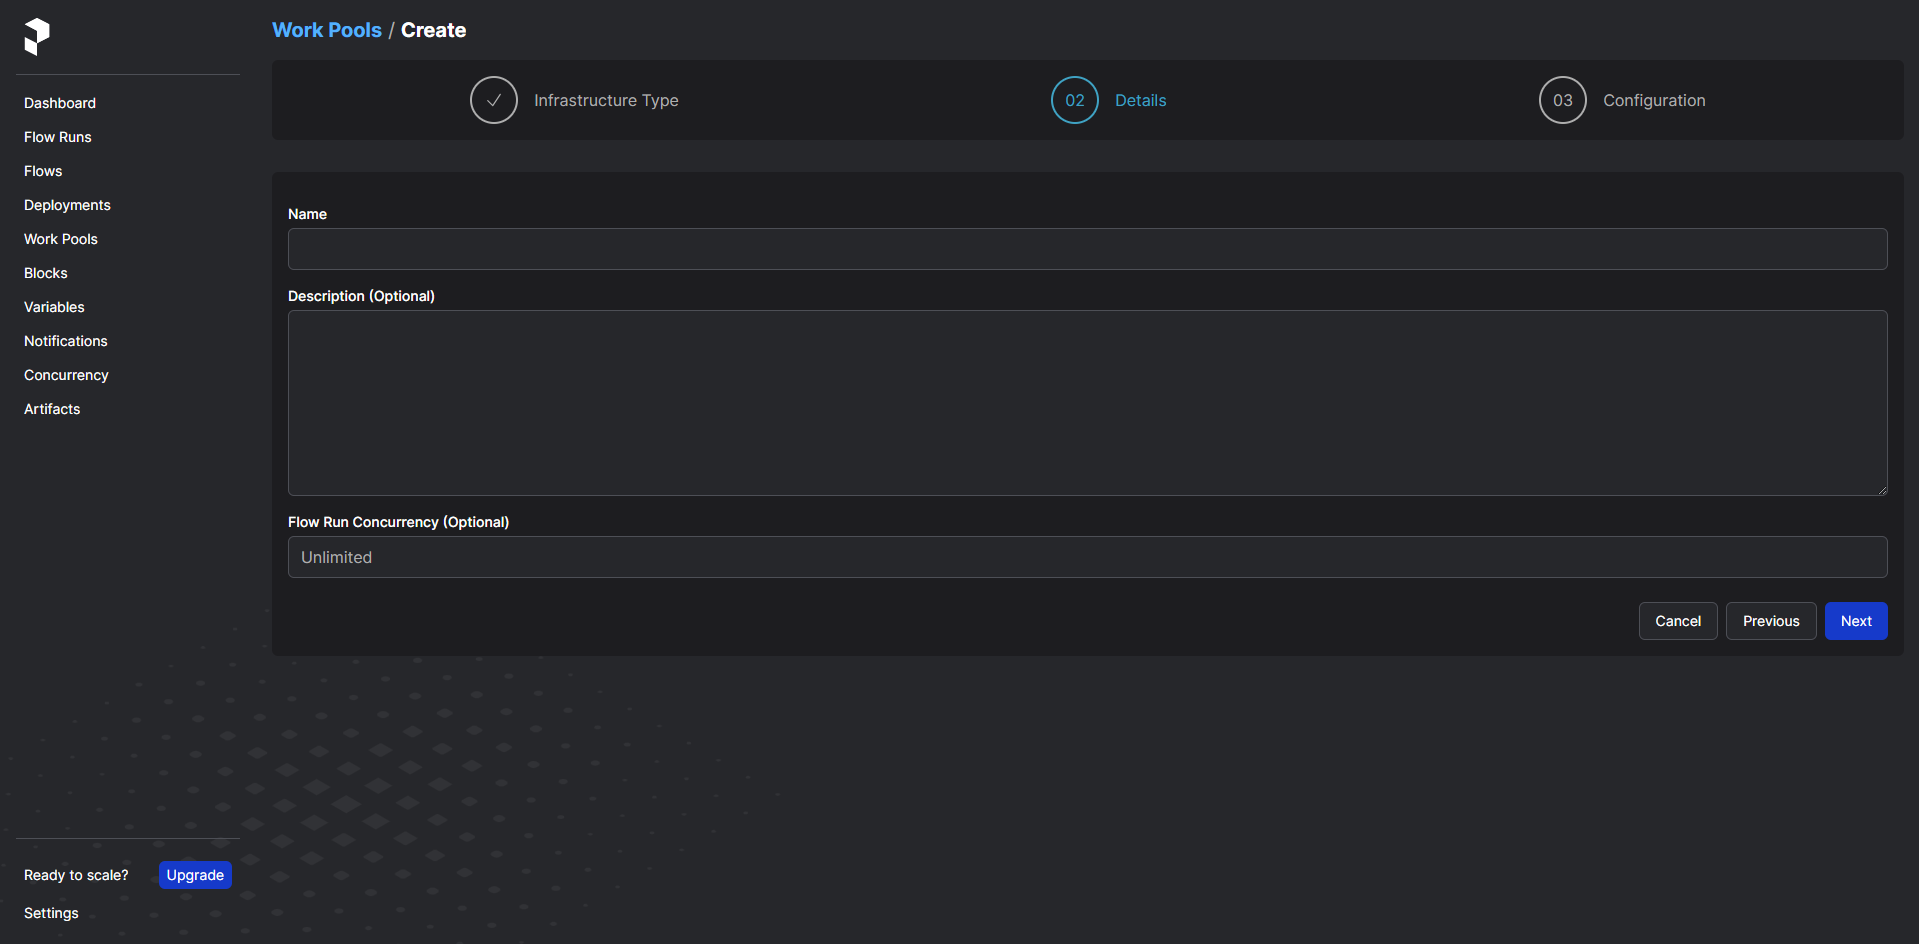
\includegraphics[width=0.9\linewidth]{graphics/Prefect_Work_Pools_Create_Details.PNG}
    \caption{Details van de create van een Prefect Work Pool}
    \label{fig:Prefect_Work_Pools_Create_Details}
\end{figure}

Op de laatste pagina worden ten slotte extra parameters ingesteld met betrekking tot de cloudprovider, zoals te zien is op Figuur~\ref{fig:Prefect_Work_Pools_Create_parameters}

\begin{figure}
    \centering
    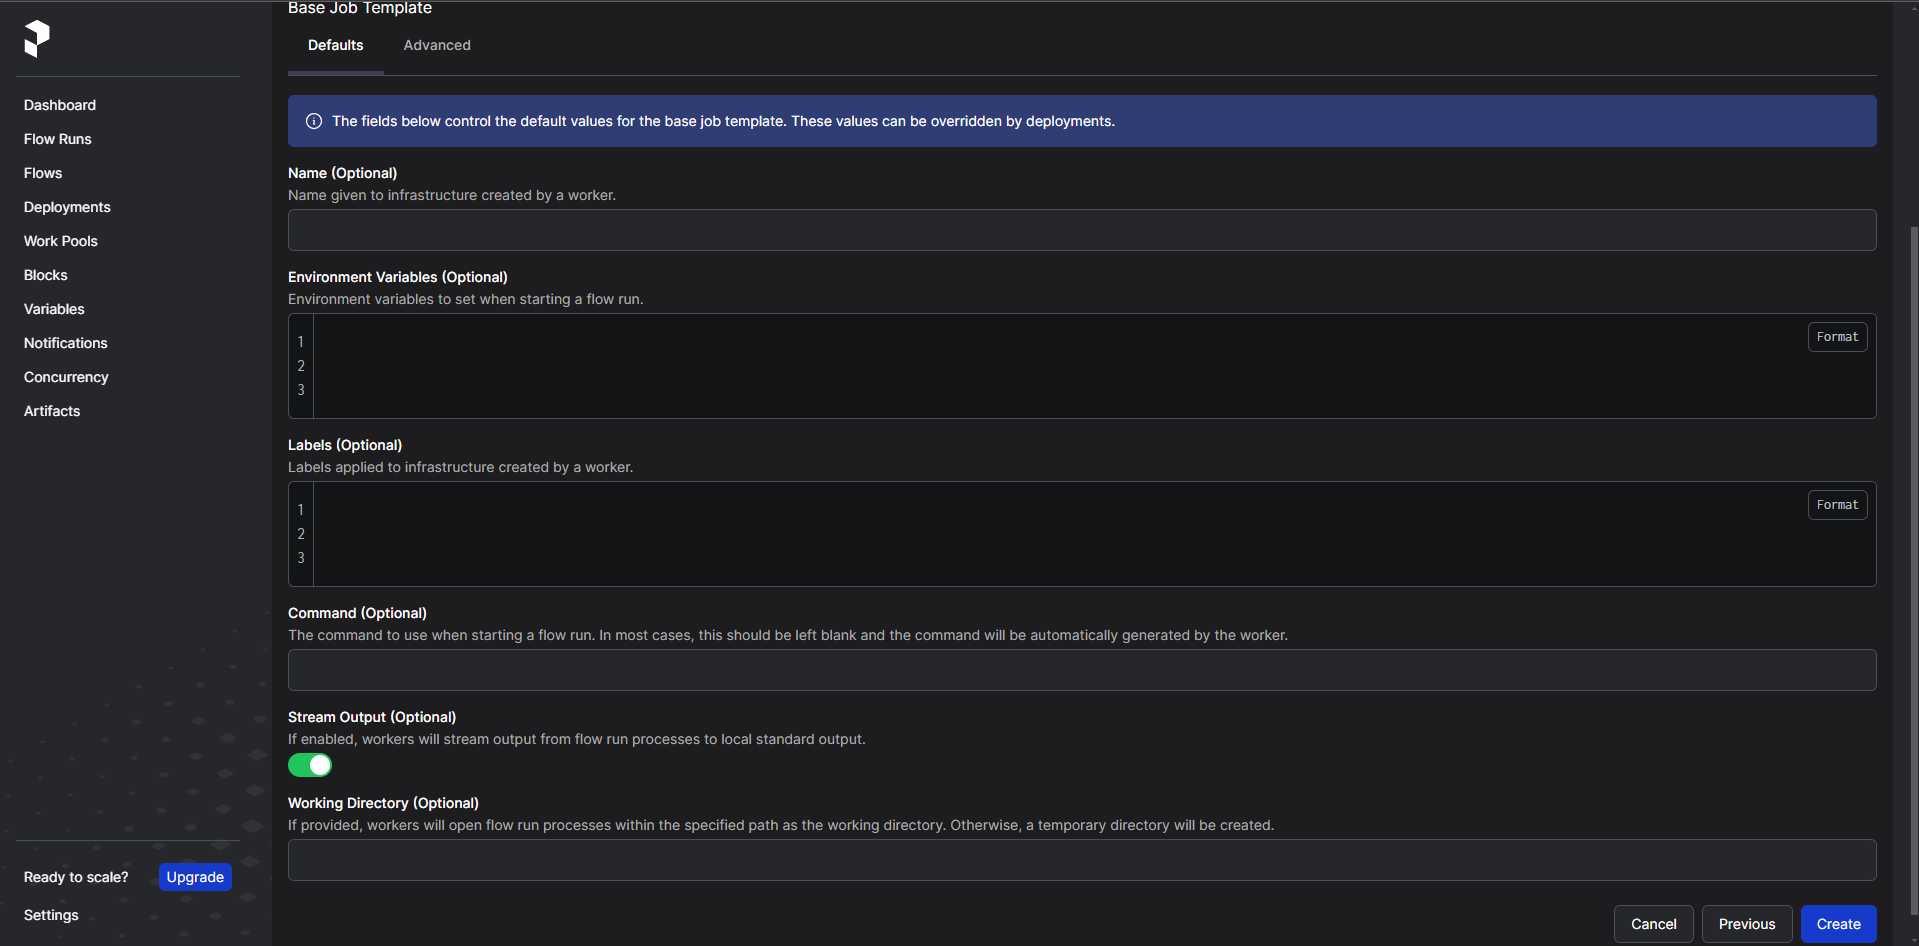
\includegraphics[width=0.9\linewidth]{graphics/Prefect_Work_Pools_Create_Parameters.PNG}
    \caption{Prefect Work Pool Creation Details}
    \label{fig:Prefect_Work_Pools_Create_parameters}
\end{figure}